% 
% Annual Cognitive Science Conference
% Sample LaTeX Paper -- Proceedings Format
% 

% Original : Ashwin Ram (ashwin@cc.gatech.edu)       04/01/1994
% Modified : Johanna Moore (jmoore@cs.pitt.edu)      03/17/1995
% Modified : David Noelle (noelle@ucsd.edu)          03/15/1996
% Modified : Pat Langley (langley@cs.stanford.edu)   01/26/1997
% Latex2e corrections by Ramin Charles Nakisa        01/28/1997 
% Modified : Tina Eliassi-Rad (eliassi@cs.wisc.edu)  01/31/1998
% Modified : Trisha Yannuzzi (trisha@ircs.upenn.edu) 12/28/1999 (in process)
% Modified : Mary Ellen Foster (M.E.Foster@ed.ac.uk) 12/11/2000
% Modified : Ken Forbus                              01/23/2004
% Modified : Eli M. Silk (esilk@pitt.edu)            05/24/2005
% Modified : Niels Taatgen (taatgen@cmu.edu)         10/24/2006
% Modified : David Noelle (dnoelle@ucmerced.edu)     11/19/2014
% Modified : Roger Levy (rplevy@mit.edu)     12/31/2018



%% Change "letterpaper" in the following line to "a4paper" if you must.

\documentclass[10pt,letterpaper]{article}

\usepackage{cogsci}
\usepackage{pslatex}
\usepackage{apacite}
\usepackage{float} % Roger Levy added this and changed figure/table
                   % placement to [H] for conformity to Word template,
                   % though floating tables and figures to top is
                   % still generally recommended!
                   
%\cogscifinalcopy % Uncomment this line for the final submission 


%\usepackage[none]{hyphenat} % Sometimes it can be useful to turn off
%hyphenation for purposes such as spell checking of the resulting
%PDF.  Uncomment this block to turn off hyphenation.

\usepackage{graphicx}
\usepackage{amsmath}
\usepackage{xcolor}

\newcommand{\tableref}[1]{Table~\ref{#1}}
\newcommand{\figref}[1]{Figure~\ref{#1}}
\newcommand{\expref}[1]{Experiment~#1}

%\setlength\titlebox{4.5cm}
% You can expand the titlebox if you need extra space
% to show all the authors. Please do not make the titlebox
% smaller than 4.5cm (the original size).
%%If you do, we reserve the right to require you to change it back in
%%the camera-ready version, which could interfere with the timely
%%appearance of your paper in the Proceedings.

\definecolor{Red}{RGB}{180,20,140}
\definecolor{Blue}{RGB}{0,0,255}
\newcommand{\jd}[1]{\textcolor{Red}{\textbf{[jd: #1]}}} 
\newcommand{\lk}[1]{\textcolor{Blue}{\textbf{[lk: #1]}}} 

\title{Seeing is believing: testing an explicit linking assumption for visual world eye-tracking in psycholinguistics} 
 
\author{{\large \bf Judith Degen (jdegen@stanford.edu)} \\
  Department of Linguistics, 450 Jane Stanford Way \\
  Stanford, CA 94305 USA
  \AND {\large \bf Leyla Kursat (lkursat@stanford.edu)} \\
  Department of Linguistics, 450 Jane Stanford Way \\
  Stanford, CA 94305 USA
  \AND {\large \bf Daisy Leigh (ddleigh@stanford.edu)} \\
  Department of Linguistics, 450 Jane Stanford Way \\
  Stanford, CA 94305 USA}


\begin{document}

\maketitle


\begin{abstract}

\jd{write}

\textbf{Keywords:} 
psycholinguistics; experimental pragmatics;  scalar implicature; linking functions; visual world; eye-tracking
\end{abstract}


\section{Introduction}

Experimental investigation is a key method of scientific inquiry in cognitive science, and experimental data has informed cognitive theory-building for centuries. A key ingredient in  using empirical data to put theories to the test is the assumption made by researchers about how the mapping between theoretical notions and empirical measurements: the \emph{linking assumption}. Indeed, empirical measurement, and the data resulting from it, are only useful and informative if the assumed linking assumption is (sufficiently) clear and justified. We argue that both clarity and justification are currently typically lacking for linking assumptions made for \emph{visual world eye-tracking}, a widely used experimental method in psycholinguistic research. We highlight the role that visual world eye-tracking has played in the burgeoning field of experimental pragmatics, which suffers particularly acutely from a lack of clear and justified linking assumptions. We then test a (usually implicitly) assumed linking assumption for referential tasks, which we term the \emph{Referential Belief} linking assumption: that the proportion of looks to a referent in a time window reflects participants' degree of belief that the referent is the intended target in that time window. To do so, we compare eye movement data against explicit beliefs collected in an incremental decision task. We make use of a previously collected eye movement dataset on scalar implicature processing \cite<\expref{3}>{sun2020}, \jd{which we also replicate in a web-based eye-tracking paradigm using \texttt{webgazer.js}  (\expref{2})}. We collect explicit beliefs to test against the original and replicated eye movement data in \expref{1}. 

\section{Linking assumptions for visual world eye-tracking}

Visual world eye-tracking (VWE) is a widely used measure in psycholinguistics, fruitfully driving advances in our understanding of phonetic, lexical, syntactic, prosodic, semantic, and pragmatic processing  \cite{tanenhaus1995,Allopenna1998,altmann1999,clayards2008,SedivyEtAl1999:Achieving-Incremental-Semantic-,huang2009,kurumada2014}. %LeffelXiangKennedy2016:Imprecision-is-Pragmatic-,}
In standard VWE tasks, participants view displays of objects while listening to spoken sentences while their eye movements are monitored (see \figref{fig:display} for an example). The popularity of VWE stems from one of its very desirable features: eye movements can be interpreted as an indicator of attention that is closely time-locked to the linguistic signal and not subject to voluntary control \jd{get ref for this}. Language can guide eye movements to a region of interest in a display within 200 ms \cite{Allopenna1998}. By sampling an x/y coordinate every few milliseconds, researchers thus obtain a very temporally fine-grained record of participants' language-directed attention over the course of an unfolding utterance. This property has been particularly useful in resolving questions regarding the time-course of online language processing, which typically cannot be addressed using offline measures like forced choice, truth-value judgments, or even more coarse-grained temporal measures like response times from button presses. Notable VWE findings that could not have been obtained with more coarse-grained measures include the diverse insights that visual context is rapidly integrated into syntactic structure assignment \cite{tanenhaus1995,chambers2004}, that words are processed incrementally and listeners maintain uncertainty about past input \cite{Allopenna1998,clayards2008}, and that listeners anticipate upcoming linguistic material based on selectional restrictions and rapid pragmatic reasoning \cite{altmann1999,SedivyEtAl1999:Achieving-Incremental-Semantic-}.

These notable successes notwithstanding, there is an elephant in the room: we still have a relatively poor understanding of how to link observed eye movements to the underlying mental processes that generate them \cite{SalverdaTanenhaus2017:The-Visual-World-Paradigm, tanenhaus2000eye, Allopenna1998, magnuson2019fixations}, a problem that is exacerbated when little attention is paid to the further variability in interpretation of eye movements introduced by the vastly different tasks employed in the literature. Consider just the difference between active referential tasks (in which participants' goal is to identify the speaker's intended referent, and frequently to select it) and passive predictive tasks (in which participants simply watch a display while listening to language, without an over task or goal). In the former case, an argument can be made that eye movements reflect listeners' active search for or belief in the referent, depending on whether visual information about the display has been integrated. In the latter case, the evidence indicates that eye movements reflect an automatic predictive process \cite{altmann1999}. But what, exactly, does this mean? What is the generative process by which, e.g., a notion like ``prediction" ultimately results in an eye movement to a region at a particular point in time? Few make clear assumptions about the generative process underlying eye movements \cite<but for a principled early example, see >{Allopenna1998}.

Here, we test an explicit linking assumption for referential tasks, which we term the Referential Belief linking assumption: that the proportion of looks to a referent in a time window reflects participants' degree of belief that the referent is the intended target in that time window. This linking assumption was tested and found not supported in previous work \cite{QingLD2018}. In a re-analysis of an experimental semantics dataset on the processing of relative and absolute gradable adjectives \cite{LeffelXiangKennedy2016:Imprecision-is-Pragmatic-}, \citeA{QingLD2018} found that explicit beliefs collected in an incremental decision task \cite<similar to gating tasks,>{Allopenna1998} did not correlate with eye movements, with the exception of one condition. They argued that the reason for the lack of support may have been participants' close to zero expectation  for observing the linguistic stimuli used in the original experiment, where expectation was linked to production probabilities elicited in a separate free production task.

Of course, it is also possible that the incremental decision task simply does not capture the beliefs that inform eye movements. We believe this is unlikely, given recent successes in using such tasks to elicit contrastive inferences \cite{KreissDegen2020, alsop2018}, but acknowledge the possibility. The previous failure to find support for the Referential Belief link, compounded by the concern regarding the validity of the incremental decision task, motivates the current study: to test the Referential Belief link on a different dataset. For this purpose, we replicate \expref{3} of \citeA{sun2020} in an incremental decision task rather than an eye-tracking task (\expref{1}) and ask how well the explicit beliefs predict the eye movement data. \jd{webgazer?}


\section{Test bed: Sun \& Breheny (2020)}

We replicate \expref{3} of \citeA{sun2020}, which addressed a now classic question in experimental pragmatics: is the processing of scalar inferences delayed relative to the processing of literal information \cite{bott2004, Breheny2006, huang2009, grodner2010, DegenTanenhaus2015, DegenT2016, Tomlinson2013}? In particular,  \citeA{sun2020} were interested in assessing the possible effect of two factors on the speed with which determiners are processed: first, pre-existing low-level associations between determiners and set sizes (i.e., a preference for \emph{all} to be associated with bigger set sizes and for \emph{some} to not show a clear preference, as established in a norming study); and second, whether the application of the determiner to a set of objects can be verified without checking a separate set of objects. For instance, the partial utterance \emph{Click on the boy that has three}, heard in the left display of \figref{fig:display}, requires only verifying that there is a boy with three objects. In contrast, replacing \emph{three} with either \emph{all} or \emph{some} requires additionally verifying that there are no other apples in the display or -- if \emph{some} is pragmatically enriched to \emph{not all} --  that there is at least one other orange in the display, respectively. That is, \emph{all} and \emph{some} should require additional processing time before settling on the target, but if \emph{some} is immediately enriched to \emph{some, but not all}, verification looks to what \citeA{sun2020} call the `residue set' (the remaining objects in the center of the screen) should increase immediately after observing the determiner. 

\begin{figure}[H]
\centering
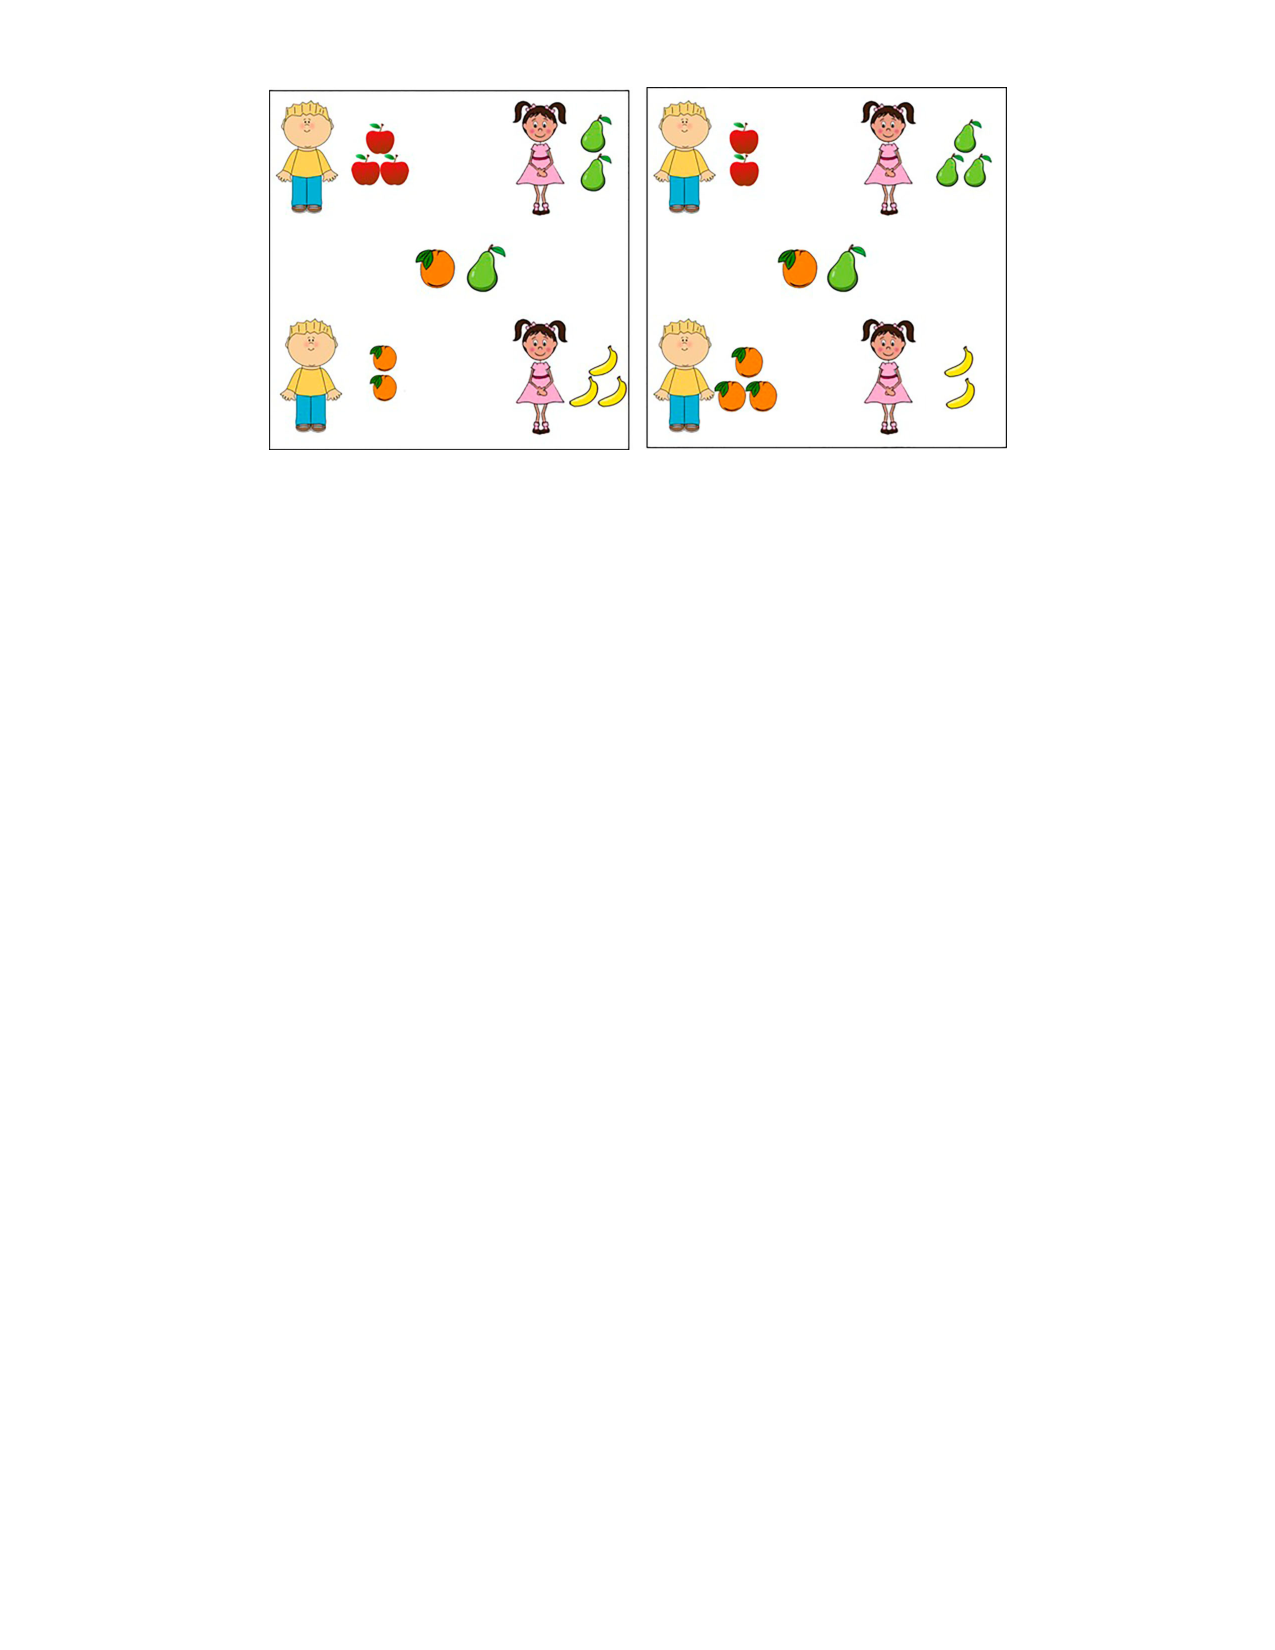
\includegraphics[width=\columnwidth]{images/display}
\caption{Example displays from \expref{3} of \citeA{sun2020}. The left image (big \emph{all}/ small  \emph{some}) was paired with  \emph{Click on the boy that has all/three of Susan's apples} or  \emph{Click on the girl that has some/two of Susan's pears}. The right image (small  \emph{all}/ big  \emph{some}) was paired with  \emph{Click on the boy that has all/two of Susan's apples} or  \emph{Click on the girl that has some/three of Susan's pears}.} 
\label{fig:display}
\end{figure}

Their predictions were borne out (see target advantage scores in  \figref{fig:results-original}). In the determiner window (200ms after determiner onset to 200ms after name onset) and the name window (200ms after name onset to 200ms after noun onset), number terms led to more (and a faster increase in) target looks than did \emph{all} and \emph{some}, suggesting that the need for verification of the residue set is a source of relatively fewer target looks for \emph{all} and \emph{some}. Moreover, while there was no effect of set size in the number or \emph{some} condition, big \emph{all} led to more target looks than small \emph{all}. Finally, and crucially for their purposes, they found that looks to the residue set in the determiner window increased for both \emph{all} and \emph{some} (but not numbers) equally and at the same time. 

Jointly, their results support what they call the fast-pragmatic account: the view that the computation of scalar inferences itself is not delayed compared to literal processing, and that previously reported apparent slowdowns in processing of \emph{some} are instead likely due to joint effects of verification time and low-level set size associations for \emph{all} which facilitate the processing of big \emph{all} compared to small \emph{some}. 


\begin{figure*}
\centering
%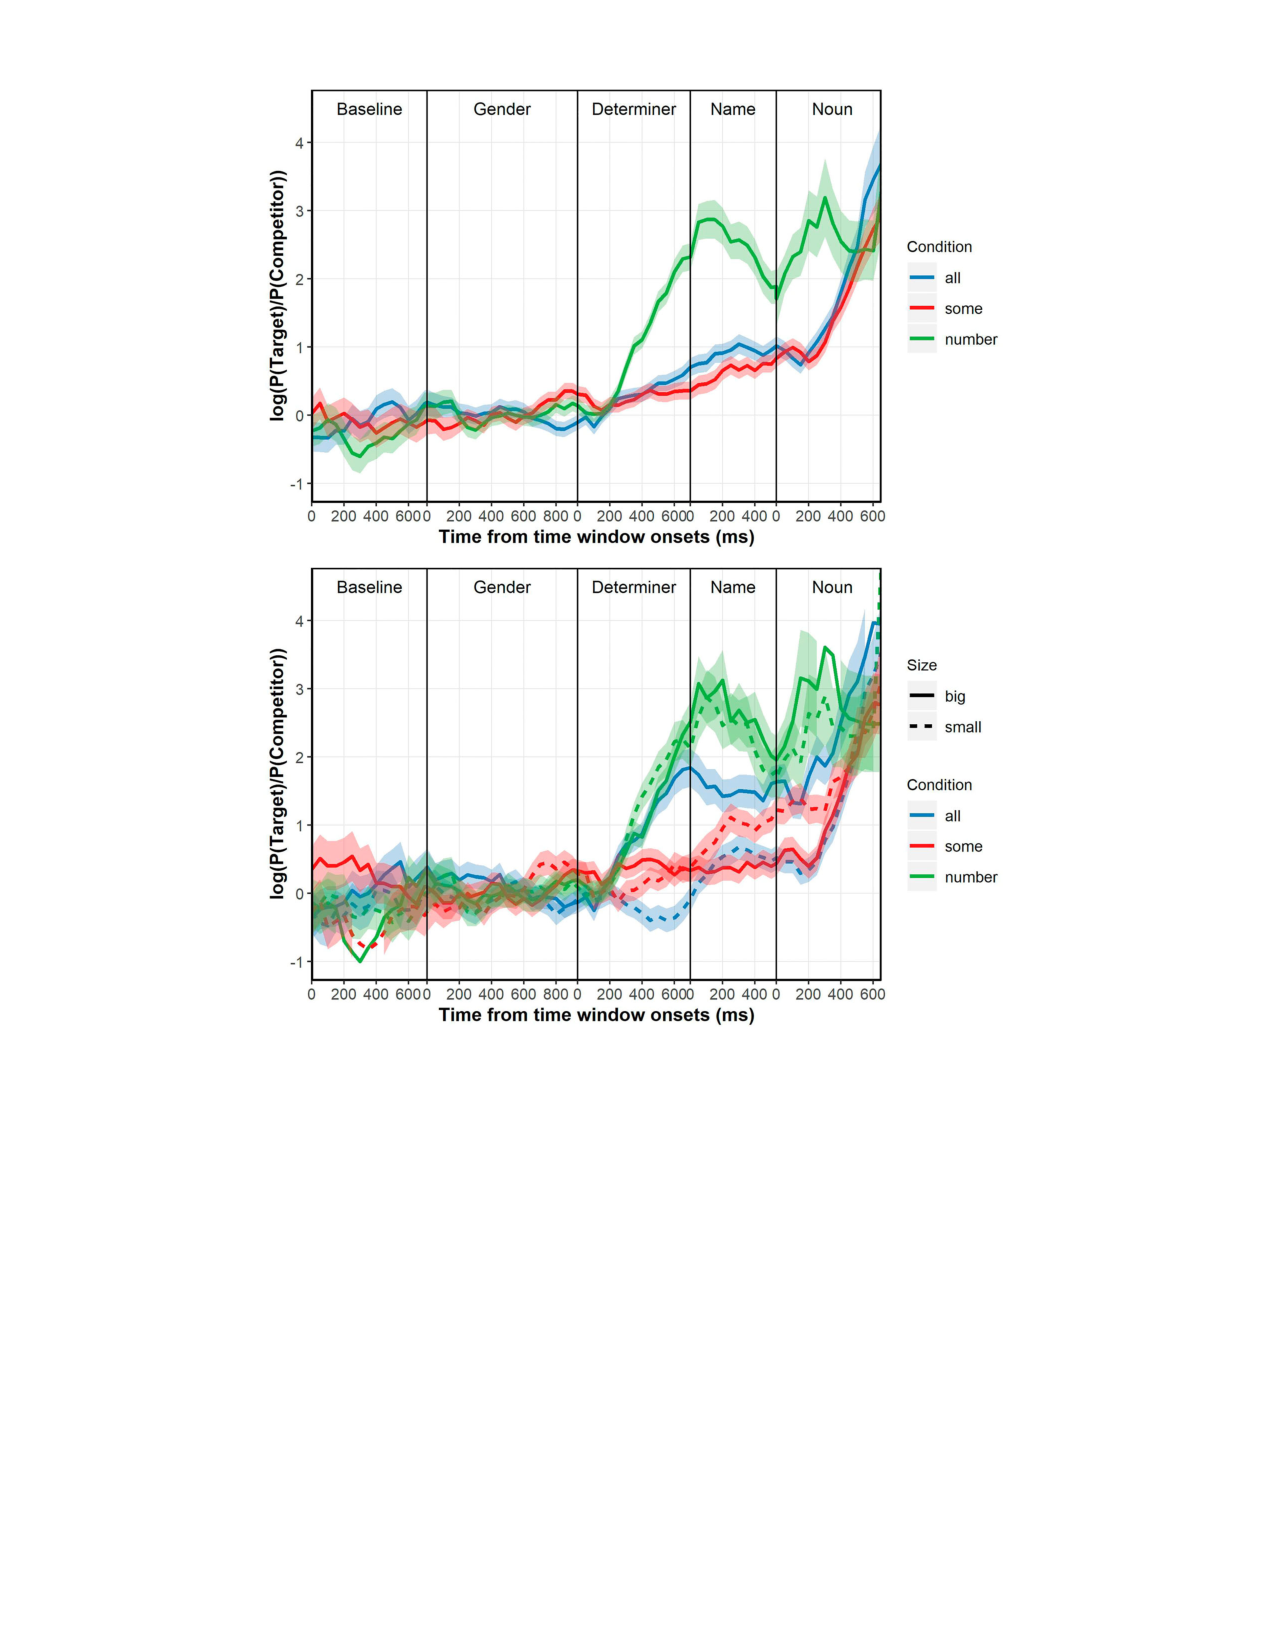
\includegraphics[width=\columnwidth]{images/results-original}
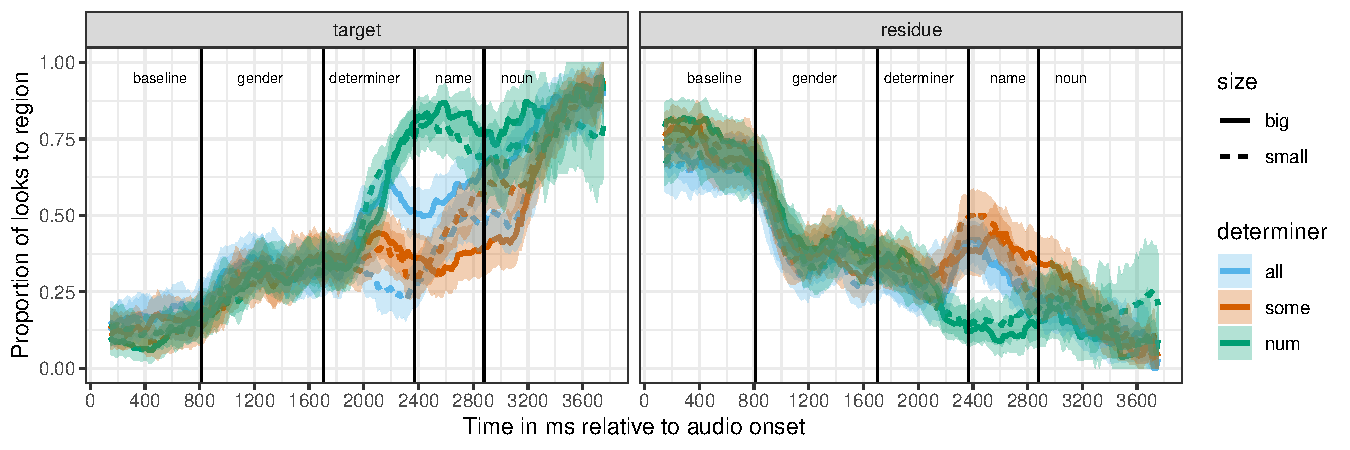
\includegraphics[width=\textwidth]{../../analysis/SunBreheny/1_incremental/main/graphs/proportions_condsize_withresidue_tr.pdf}
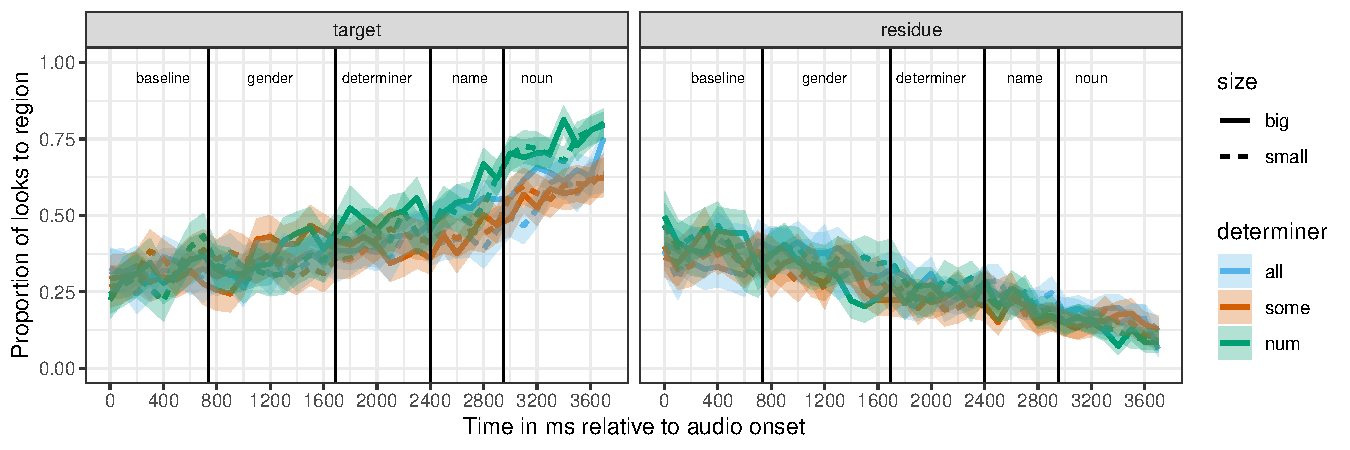
\includegraphics[width=\textwidth]{../../analysis/SunBreheny/2_webgazer/main/graphs/proportions_condsize_withresidue_tr.pdf}
\caption{Proportion of looks (out of target, competitor, and residue looks) to target (left) and residue (right) from instruction onset. Transparent ribbons indicate 95\% bootstrapped confidence intervals. Black vertical lines indicate onsets of analysis windows of interest (window labels at top of graphs). \textbf{Top:} \expref{3} of \citeA{sun2020}. \textbf{Bottom:} Our \expref{2}.}
\label{fig:results-original}
\end{figure*}

For the purpose of testing the Referential Belief linking assumption, this study has both appealing features as well as one glaring problem. The appealing features include the simple 2x3 design, a limited and clearly defined set of referents in each display, and the clarity of the referential task. The glaring problem, which disqualifies the Referential Belief link as a full linking theory from the outset, are the systematic looks to the residue set: the Referential Belief link is only defined for looks to possible referents. There is no plausible argument to be made that participants look to the residue set because they believe it may be the intended target.  Thus, we have already identified one way in which, if otherwise supported by the data, the Referential Belief link will have to be extended. We return to this point in the General Discussion.


\section{Exp.~1: replicating Sun \& Breheny (2020) using an incremental decision task}

In order to measure participants' beliefs about the intended referent at points in the utterance that would allow us to compare explicit beliefs to proportions of looks in \citeA{sun2020}, participants engaged in an incremental decision task \cite{Allopenna1998,QingLD2018, KreissDegen2020,alsop2018}. 

\subsection{Methods}

\textbf{Participants.} We recruited 120 participants on Mechanical Turk, of which \jd{XXX} were excluded because \jd{X Y, Z}. 

\textbf{Materials and procedure.} We measured participants' beliefs about the intended referent for each display shown to participants by \citeA{sun2020} (see \figref{fig:display} for examples). Participants were told that they were playing a guessing game, and whenever they made a guess, more words would appear. The critical sentences of the form ``Click on the GENDER who has DETERMINER  of NAME's NOUN" were revealed incrementally. GENDER was one of \emph{boy/girl}, DETERMINER was one of \emph{some/all/two/three}, NAME was one of \emph{Susan/Amy/Michael}, and NOUN was one of \emph{apples/bananas/erasers/scissors/knives/rulers/forks/plates/
spoons/pencils/pears/oranges}.  Participants clicked on the presumed target after (a) ``Click on the" (baseline window), (b) ``GENDER that has" (gender window), (c) ``DETERMINER of NAME's" (determiner window), and (d) ``NOUN" (noun window). After each click, the next word(s) or display was shown. After 6 practice trials, each participant saw 48 experimental trials, of which 12 were filler trials with the number terms \emph{one} and \emph{four}. The 36 critical trials implemented \citeA{sun2020}'s 2 (big vs.~small target set) by 3 (\emph{all, some}, number) design. 


\subsection{Results}

%Following \citeA{sun2020}, we computed the target preference score $\ln (\frac{p(\text{target})}{p(\text{competitor})})$ for each time window, where  $p(\text{target})$ and $p(\text{competitor})$ refer to the proportion of target and competitor selections, respectively (see \figref{fig:results-idt}). Proportions were aggregated by subject, determiner, and set size. 

\figref{fig:results-idt} shows proportions of target selections out of all selections in each time window and condition. 


\textbf{Data analysis}. \citeA{sun2020} fit separate linear regression models to target advantage scores in time windows of interest. We instead fit logistic mixed effects models predicting target selections. This choice was motivated by logistic regression being the more principled approach to modeling categorical data. It also avoids the problems of having to pre-aggregate data and add smoothing terms to avoid division by zero (or having to discard mathematically problematic data points all together). \jd{The results are qualitatively identical if we instead run linear models on target preference scores. (??)}

\citeA{sun2020} fit separate models to the baseline, gender, determiner, name, and noun windows. We collapsed the name window into the determiner window because the name does not add disambiguating information. The models predicted target over competitor choices from fixed effects of quantifier (reference level: ``number"), centered size (higher value: ``big"), by-item and by-subject random intercepts, and random by-subject slopes for condition and size. No effects reached significance in the baseline, gender, and noun window, as expected.\footnote{In fact, fitting models to the noun window was impossible because participants, with very few exceptions, always chose the target. That is, there was no variance to speak of that a model could be estimated to explain.}  In the determiner window, the window of interest, there were main effects of condition, such that target selections were less likely in both the \emph{some} ($\beta$=-2.90, $SE$=0.36, $p<$.0001) and \emph{all} ($\beta$=-2.92, $SE$=0.36, $p<$.0001) conditions, compared to the number condition. There was no main effect of size, consistent with the visual result that target selections in the number condition are not modulated by  target set size ($\beta$=-0.09, $SE$=0.26, $p<$.73). However, we did observe interactions between quantifier and size, such that small sets resulted in more target selections for \emph{some} ($\beta$=0.59, $SE$=0.28, $p<$.05) but fewer target selections for \emph{all} ($\beta$=-1.27, $SE$=0.29, $p<$.0001), compared to number terms. 

%(Intercept)          3.77254    0.39655   9.513  < 2e-16 ***
%conditionall        -2.92409    0.36359  -8.042 8.81e-16 *** 		replicates
%conditionsome       -2.90211    0.36217  -8.013 1.12e-15 ***		replicates
%csize               -0.09207    0.26069  -0.353   0.7239    			does not replicate -- they found main effect (more looks to big set and steeper increase)
%conditionall:csize  -1.27305    0.28523  -4.463 8.08e-06 ***		replicates
%conditionsome:csize  0.59465    0.27945   2.128   0.0333 *  		does not replicate , they found null effect (but perhaps in name window? they don't report this specifically)

\begin{figure}[H]
\centering
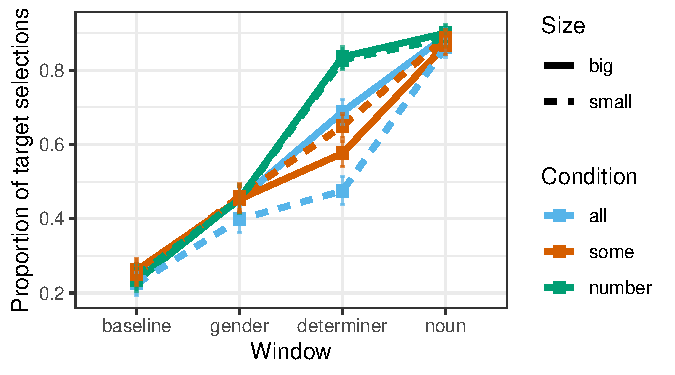
\includegraphics[width=\columnwidth]{../../analysis/SunBreheny/1_incremental/main/graphs/results-target-all-looks}
%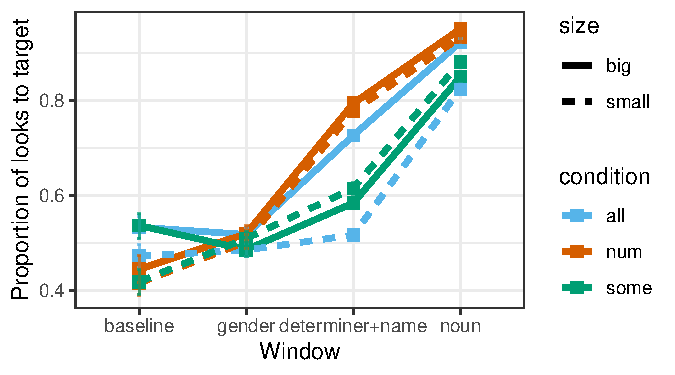
\includegraphics[width=\columnwidth]{../../analysis/SunBreheny/1_incremental/main/graphs/results-target}
%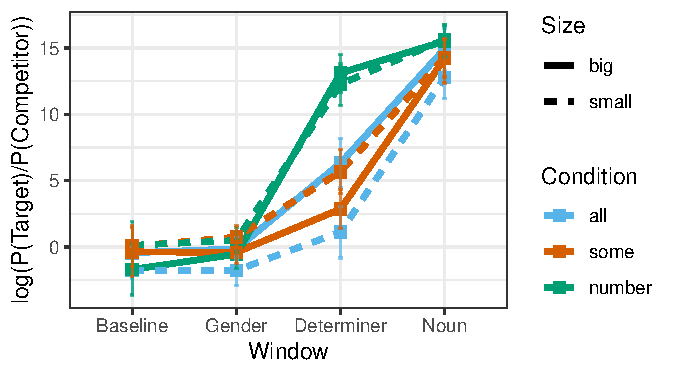
\includegraphics[width=\columnwidth]{../../analysis/SunBreheny/1_incremental/main/graphs/results-idt}
\caption{Proportion of target selections in \expref{1} by quantifier and set size. Error bars indicate 95\% bootstrapped confidence intervals.} 
\label{fig:results-idt}
\end{figure}

\textbf{Comparison with \citeA{sun2020}: replication analysis}. These results constitute a near-perfect replication of  \citeA{sun2020}. Most of their effects reported in the determiner window replicated, with two exceptions: we did not observe a main effect of set size, while they did; and we observed an interaction of size and determiner such that small \emph{some} led to greater target selections than big \emph{some}. These differences are not as big as they may seem: in our dataset, the lack of set size main effect can be explained by the interactions with determiner: while size makes no difference at all for number (the determiner predictor reference level), it has the opposite effect for \emph{all} compared to \emph{some}. A similar tendency can be observed in  \citeA{sun2020}'s results when taking into account the joint determiner and name windows. In fact,  \citeA{sun2020} report the absence of a main effect for size in the name window, and instead an interaction between size and determiner. While they do not report the same post hoc analyses, visual inspection of \figref{fig:results-original} suggests that the interaction in the name window is indeed the result of set size having the opposite effect for \emph{all} compared to \emph{some}. Thus, when taking into account their results from both the determiner and name window, which we collapsed into one, the results are qualitatively identical. The different results reported by  \citeA{sun2020} in the two time windows are presumably the result of certain information taking longer to be integrated, something which the incremental decision task by its offline nature cannot capture. \jd{if time, re-analyze their results with logistic models?}

\textbf{Comparison with \citeA{sun2020}: linking function analysis}. For the purpose of evaluating the Referential Belief link, we conduct correlational analyses at different levels. The overall correlation between proportion of selections in \expref{1} and proportions of looks in \citeA{sun2020} at the item level, i.e., where proportions were calculated separately by region of interest (target, competitor, distractors), time window (baseline, gender, determiner$+$name, noun), determiner (\emph{all, some}, number), set size (big, small), and noun, was high ($r(862) = .87$, $p < .0001$). More interesting than inspecting the overall correlation, however, is to investigate the conditions under which explicit and implicit beliefs are more and less closely aligned. For this purpose, we examined the correlations by time window (see \figref{fig:corr-window}), for the determiner window of interest by condition  (see \figref{fig:corr-determiner}), and by region of interest  (see \figref{fig:corr-region}).


\begin{figure*}
\centering
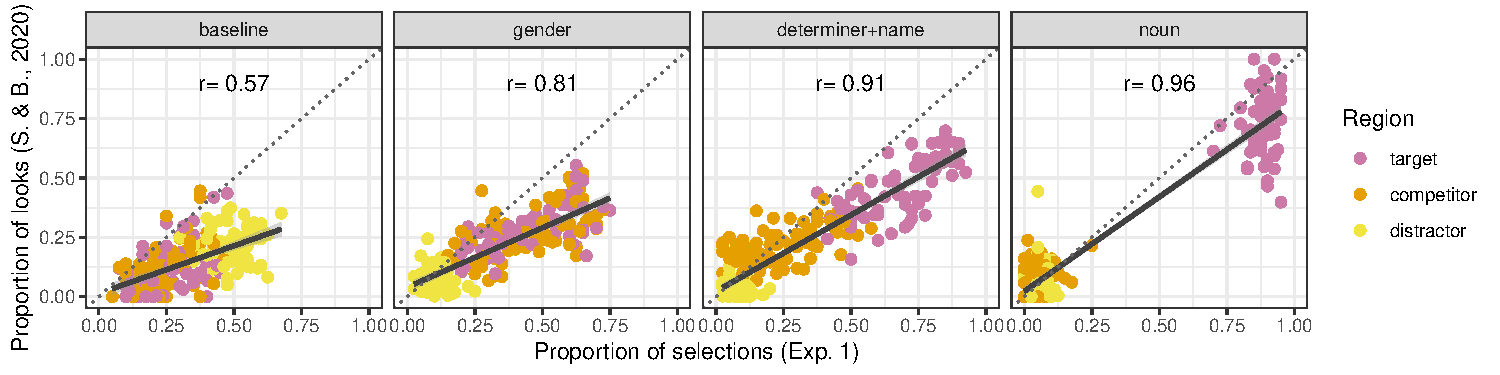
\includegraphics[width=.9\textwidth]{../../analysis/SunBreheny/1_incremental/main/graphs/corr-window}
\caption{Proportions of looks in \citeA{sun2020} against proportions of selections in \expref{1}. Facets indicate time windows.} 
\label{fig:corr-window}
\end{figure*}


%Correlation between proportion of target selections in determiner window and target looks in determiner\+name window: Pearson's $r=.99$. Competitor: $r=.86$. Distractors: $r=.93$.

\jd{CONTINUE HERE DESCRIBING LINKING FUNCTION RESULTS}

%\begin{figure}[H]
%\centering
%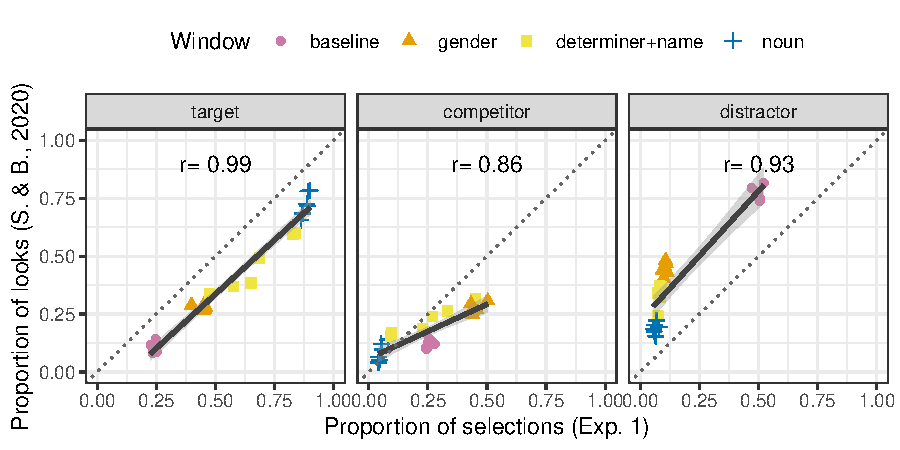
\includegraphics[width=\columnwidth]{../../analysis/SunBreheny/1_incremental/main/graphs/correlations}
%\caption{Proportions of looks in \citeA{sun2020} against proportions of selections in \expref{1}. Facets indicate regions, colors indicate time window.} 
%\label{fig:results-correlations}
%\end{figure}
%
%\begin{figure}[H]
%\centering
%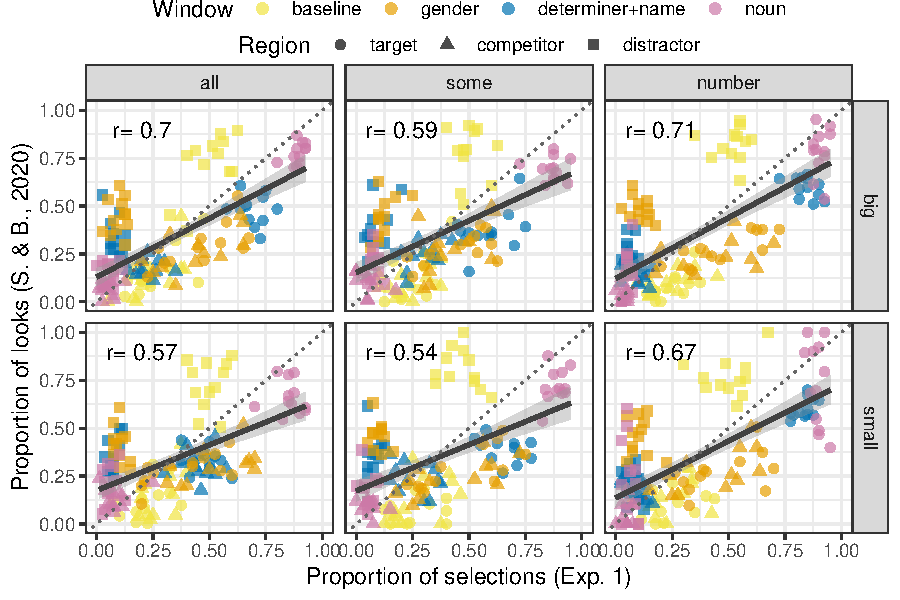
\includegraphics[width=\columnwidth]{../../analysis/SunBreheny/1_incremental/main/graphs/correlations-bycondition}
%\caption{Proportions of looks in \citeA{sun2020} against proportions of selections in \expref{1}. Facets indicate regions, colors indicate time window.} 
%\label{fig:results-correlations}
%\end{figure}

\section{Exp.~2 \jd{fix all refs}: replicating Sun \& Breheny (2020) using web-based eye-tracking}

\jd{\dots will it work? tbd.}

\subsection{Methods}

\textbf{Participants.} We recruited 183 participants on Prolific, of which 21 were excluded because their accuracy was lower than 95\%. We also excluded trials on which the participants clicked the wrong target (33 trials). All participants were self-reported native English speakers.\footnote{Procedure, materials, analyses and exclusions were pre-registered at https://osf.io/y2cgb. The collected sample size for Exp.~1 (183 participants) was larger than the originally pre-registered sample size (102 participants) because 40\% of the initally tested 102 participants had a technical issue and weren't able to see the whole display. \lk{added prereg footnote here}}

\textbf{Materials and procedure.} Exp. 1 was identical to \citeA{sun2020}'s Exp. 3 except for one difference: we collected eye movements with webcam eyetracking using the webgazer library. Participants were presented with the same experimental displays as the original experiment (\figref{fig:display}). One second after the display onset, paricipants heard the auditory instruction of the form "Click on the GENDER who has DETERMINER of NAME's NOUN". Their task was to select the correct image according to the instuction. After each click, participants moved to the next trial. At the beginning of the experiment, there were 6 practice trials which familiarized participants with the characters and the task. After the practice trials, participants saw 36 critical trials and 12 fillers in randomized order. The critical trials had two (target size: big, small) by three (determiner: all, some, number) design. On each trial, eye movements were recorded from the onset of the display until the participant made a selection.

\subsection{Results}
\jd{xxx}


\section{General discussion}

\begin{itemize}
	\item main point: in contrast to previous re-analysis of leffel et al, clear support for the Referential Belief link. reasons? 
	\begin{itemize}
		\item most likely: participants in SB expected the observed language (see preliminary production results from Qing et al, but also Kreiss and Degen 2020 results, plus tons of other literature supporting tight link between production and comprehension in general, and importance of clearly nameable items (ie, clear production expectations) for VW eye-tracking in particular (go back to mike's papers from the oughts)
		\item possibly more power in SB than Leffel
	\end{itemize}
	\item pick the residue set issue back up -- possible extensions of Referential Belief link?
	\item linking function issue is a problem not just with eye-tracking but with experimental measures in xprag in general (see eg the tvjt literature, though there have been several recent attempts to be explicit abt link, especially with the advent of probabilisitc models that make specifying a clear link easier): \cite{Jasbi2019, WaldonDegen2020, franke2014typical, savinelli2018, franke2016link, scholler2017semantic, tessler2019language}
	\item methodological points:
		\begin{itemize}
			\item further validation of incermental decision task as useful measure of comprehension
			\item The additional replication suggests that web-based eye-tracking using the webgazer library is a) feasible; and b) a faster, cheaper way to collect eye movement data despite the added noise.
		\end{itemize}
	\item theoretical connection: more fine-grained RSA story that can capture the pref for small over big "some" despite "some" being bad for both; goes beyond (against?) the simple (SB and degen tanenhaus 2015/2016) production expectation story that only takes into account the probability of "some" being used for the bigger vs the smaller set. if we apply RSA, where what matters to interpretation is not just the relative probability of "some" being used for one vs the other set size, but it also matters how likely "all" and other alternatives are for the set sizes under consideration, then I think this result is expected as long as we assume that "all" is generally highly dispreferred for the small set and highly preferred for the big set. see example numbers below (assuming a uniform prior), where S is the pragmatic speaker and L is the pragmatic listener:
\end{itemize}

Hypothetical speaker distribution for small set:
\begin{eqnarray*}
S("two"|small) = .8\\
S("three"|small) = 0\\
S("all"|small) = .05\\
S("some"|small) = .15\\
\end{eqnarray*}

Hypothetical speaker distribution for big set:
\begin{eqnarray*}
S("two"|big) = 0\\
S("three"|big) = .6\\
S("all"|big) = .3\\
S("some"|big) = .1\\
\end{eqnarray*}

The above speaker assumptions result in (observed) small target advantage for small-some over big-some:
\begin{eqnarray*}
L(small|"some") =  \frac{S("some"|small)}{(S("some"|small) + S("some"|big))} \\
= .15 / (.15+.1) = .6\\
L(big|"some") = \frac{S("some"|big)}{(S("some"|small) + S("some"|big))} \\
= .1 / (.15+.1) = .4
\end{eqnarray*}

The above speaker assumptions result in (observed) large target advantage for big-all over small-all:
\begin{eqnarray*}
L(small|"all") = \frac{S("all"|small)}{(S("all"|small) + S("all"|big))}\\ 
= .05 / (.05+.3) = .14\\
L(big|"all") = .3 / (.05+.3) = .86
\end{eqnarray*}

Numbers behave categorically (assuming exact semantics):
\begin{eqnarray*}
L(small|"two") = 1\\
L(big|"two") = 0\\
L(small|"three") = 0\\
L(big|"three") = 1
\end{eqnarray*}

\dots of course this all just captures the categorical belief data and can't handle verification (eg looks to residue set) at all; must bridge to algorithmic level

%\begin{table}[H]
%\begin{center} 
%\caption{Sample table title.} 
%\label{sample-table} 
%\vskip 0.12in
%\begin{tabular}{ll} 
%\hline
%Error type    &  Example \\
%\hline
%Take smaller        &   63 - 44 = 21 \\
%Always borrow~~~~   &   96 - 42 = 34 \\
%0 - N = N           &   70 - 47 = 37 \\
%0 - N = 0           &   70 - 47 = 30 \\
%\hline
%\end{tabular} 
%\end{center} 
%\end{table}


%\begin{figure}[H]
%\begin{center}
%\fbox{CoGNiTiVe ScIeNcE}
%\end{center}
%\caption{This is a figure.} 
%\label{sample-figure}
%\end{figure}


%\section{Acknowledgments}
%
%Madigan, Daisy; chao sun and richard breheny for generously sharing materials, data


\bibliographystyle{apacite}

\setlength{\bibleftmargin}{.125in}
\setlength{\bibindent}{-\bibleftmargin}

\bibliography{sunbrehenyreplication}

\end{document}
